\section{Robótica Móvel\label{sec:robos}}

Um \textit{robô móvel}, como o nome sugere, tem a habilidade de se locomover. São contrastantes com os chamados \textit{robôs industriais}, ou \textit{robôs de manipulação com base fixa}, comumente aplicados em grandes indústrias como soluções de automação --- potentes braços mecânicos empregando movimentos repetitivos, como a montagem de automóveis, aviões, montagem de componentes eletrônicos, pintura e outros.  São diversos os tipos de robôs móveis: podem viajar em ambientes fechados, no solo, na superfície de fluidos, por baixo de fluidos, no ar e até no espaço. Essa capacidade de mobilidade fez destes soluções para vários problemas complicados de engenharia, elevando consideravelmente a pesquisa da área nas últimas décadas \cite{mobileRobotsCook}.
\\

Existem várias classificações diferentes para robôs móveis \cite{mobileRobotsTzafestas} (veja a Figura~\ref{fig:robosmoveis}). Robôs terrestres são distinguidos principalmente por \textit{Robôs Móveis com Rodas} (WMRs, do inglês \textit{Wheeled Mobile Robots}) e \textit{Robôs Móveis com Pernas} (LMRs, de \textit{Legged Mobile Robots}). Também existem os \textit{Veículos Aéreos Não Tripulados} (VANTs, ou UAVs de \textit{Unmanned Aerial Vehicles}, popularmente conhecidos como \textit{drones}) e os \textit{Veículos Subaquáticos Autônomos} (AUVs, de \textit{Autonomous Underwater Vehicles}). 

\begin{figure}[H]
	\begin{center}
		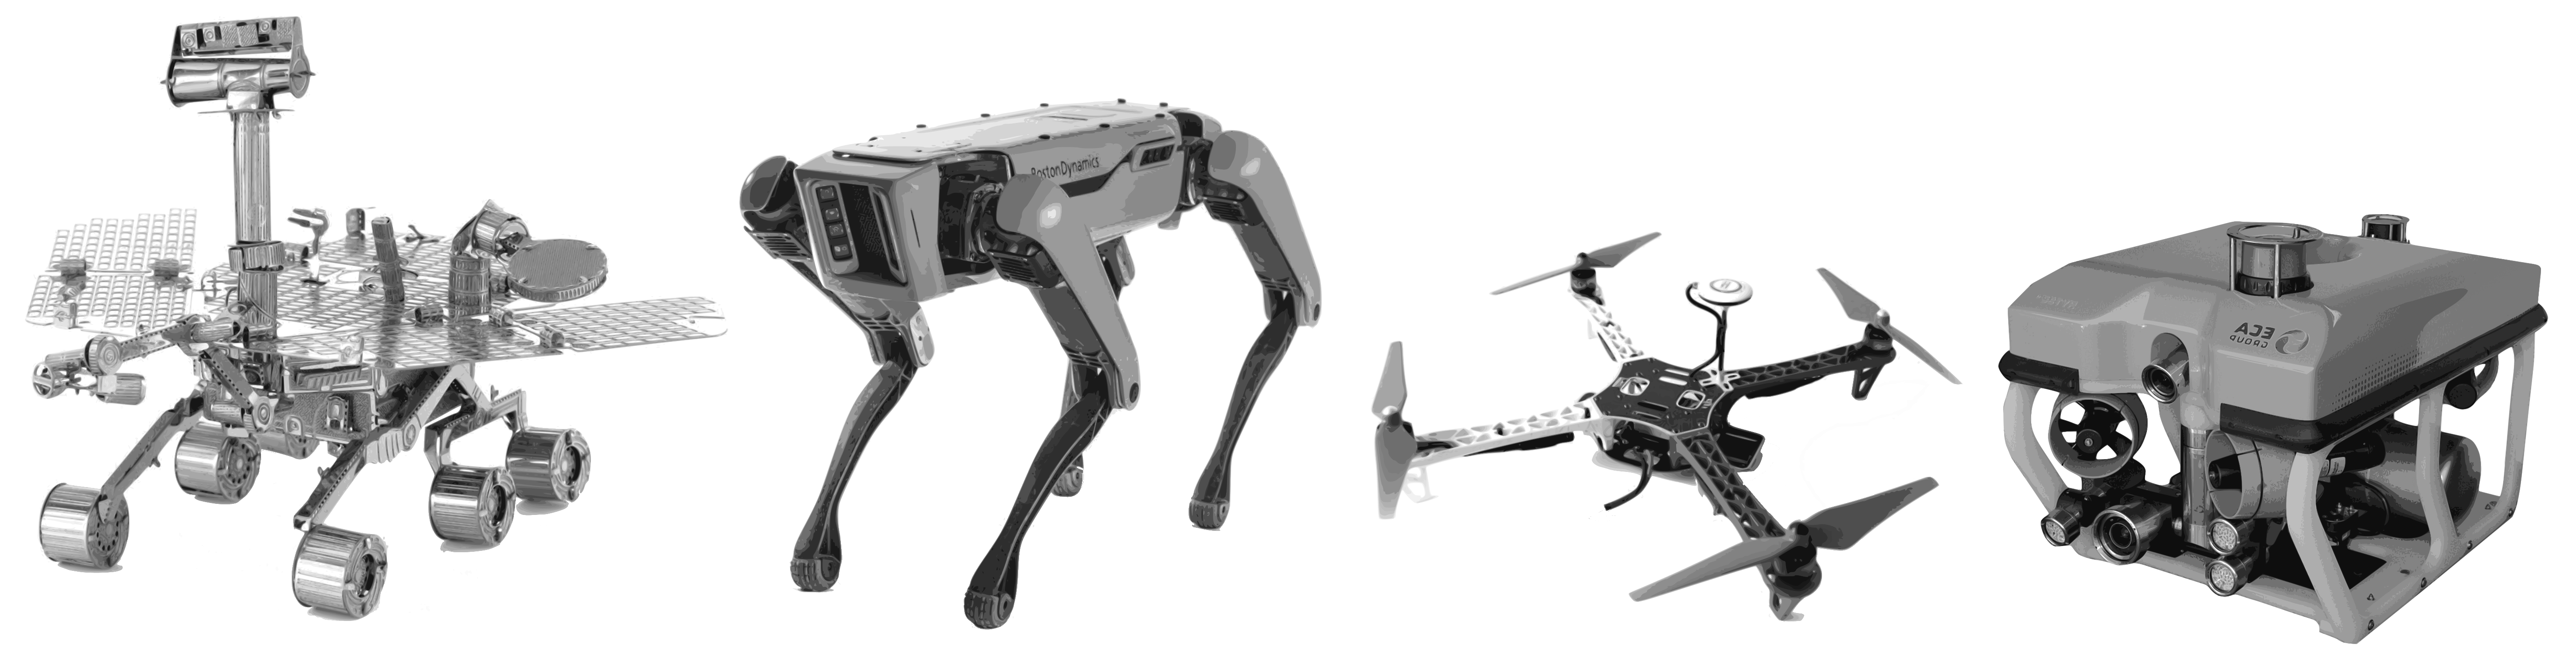
\includegraphics[width=1\linewidth]{secRobosMoveis/figures/robos.png}
	\end{center}
	\caption{Exemplos de robôs móveis. Em ordem: Um WMR usado para navegar pelo terreno de marte; Um LMR que imita o comportamento canino; Um VANT, drone com quatro hélices; Um AUV usado em elevadas profundezas marítimas.}
	\label{fig:robosmoveis}
\end{figure}

Os WMRs são muito populares devido sua baixa complexidade mecânica e pouco consumo de energia \cite{mobileRobotsWheeled}, porém, os VANTs ganharam parte interessante do mercado devido o barateamento pela fabricação em escala industrial e grande interesse da população. Há empresas, por exemplo, aplicando a utilização de VANTs como soluções de logística para entregas \cite{dronesAmazon}. Uma interessante apresentação histórica da evolução dos robôs móveis é feita em \cite{mobileRobotsTzafestas}.

De qualquer forma, como nesse texto tem-se um interesse geral por robôs móveis, não necessariamente limitados a uma aplicação específica, recorrentemente os abstrairemos como \textit{sensores}. Veja, como geralmente robôs móveis devem executar suas tarefas de forma autônoma, é de extrema importância para sua supervisão, funcionamento e controle o conhecimento de suas posições \cite{mobileRobotsCook}. Uma vez que estabelece-se uma coordenada de destino, é de extrema importância que estes utilizem de seus conjuntos de sensores para se localizar e estabilizar sua navegação.

\subsection{Sensores}
Variados tipos de sensores são comumente empregados para auxiliar na locomoção de robôs \cite{sensorsForMobileRobots}. Existem sensores de controle local, que auxiliam na locomoção do robô, garantindo que este se mantenha no melhor trajeto e não cause danos a si mesmo ou ao ambiente ao seu redor; e existem os sensores de controle global, que orientam o robô no espaço.
\begin{itemize}
	\item \textbf{Controle Local}
	\subitem \textbf{À distância:} Utilizados para determinar a presença (e estimar distância) de obstáculos e objetos sólidos no geral. Pode-se mencionar sensor infra-vermelho, de ultrassom, radar, radar laser e sistemas de visão computacional como exemplos; 
	\subitem \textbf{Por contato ou proximidade:} Informam a presença de um objeto ao alcance do robô. Alguns exemplos são bumbers, switches, animal whiskers, sensores eletromagnéticos, indutivos e capacitivos.
	\subitem \textbf{De deslocamento e velocidade:} Possibilitam a predição da posição e orientação \textit{relativa} do robô. Sensores de inércia (giroscópio e acelerômetros), odômetros (encoders ópticos ou por contato; contadores de giro), sensores de efeito doppler, trilateração não ancorada e sensores baseados em visão computacional também são comuns.
	\item \textbf{Controle Global}
	\subitem \textbf{De posição e orientação: } Determinam a posição e orientação \textit{absoluta} do robô. Módulos de GPS (Sistema de Posicionamento Global, trilateração por satélites), bússolas, módulos de trilateração usando âncoras, visão computacional (indoor) e guias fixas pré-estabelecidas (como faixas pintadas no chão) são técnicas muito empregadas.
\end{itemize}

Nota-se que visão computacional pode ser aplicada para resolver vários dos problemas de engenharia envolvendo navegação autônoma. De fato, é com essa técnica que muitos dos animais se baseia para a locomoção. Infelizmente, esta ainda é uma solução muito custosa computacionalmente, se tornando inviável para a muitas aplicações embarcadas \cite{bayro2010geometric} e que necessitam de um controle em tempo real (críticas).
\\

Em específico, nesse texto, interessa aplicar conceitos de Geometria de Distâncias no controle de \textit{posicionamento absoluto} de um robô móvel. Para isso, baseando em \cite{eren2004rigidity} e \cite{savvides2001dynamic}, define-se o problema como um grafo ponderado $G = (V,E,d)$, onde $V$ é formado pelo conjunto de sensores no espaço e $E$ define o conjunto de sensores que estão hábeis a se comunicar, respeitando suas limitações, e as distâncias entre si.

\subsection{Como medir distâncias\label{sec:sensores}}

Os métodos mais populares para estimar distância entre dois sensores são \cite{savvides2001dynamic}: \textit{Indicador de força de sinal recebido} (RSSI, de \textit{Receibed Signal Strenght Indicator}) e \textit{Métodos baseados em tempo}.
\\

\subsubsection{Intensidade de Sinal}
Seja por fio ou não, a comunicação entre sensores móveis é feita por ondas eletromagnéticas que tem sua potência alterada entre o envio e recebimento. Isso se dá pois a intensidade de um sinal eletromagnético $I$ é definido como a potência da fonte $P$ sobre área de propagação $A$, i.e., $I = \frac{P}{A}$ \cite{moysesEletromag}. Supondo que se utilize comunicação sem fio, então o sinal é propagado pelo ar em todas as direções. Como estamos no $\mathbb{R}^3$, a área de propagação do sinal é a superfície da esfera com centro na fonte, ou seja, 
$$ A(r) = 2\int_0^{\frac{\pi}{2}} 2\pi\; r^2 \cos(\theta) \; d\theta \ = \ 4\pi r^2 \ \Rightarrow \ I = \frac{P}{4\pi r^2} $$
Por tanto, a intensidade de sinal recebido é inversamente proporcional ao quadrado da distância entre a fonte do sinal e o receptor. Fixando a potência do transmissor e medindo a intensidade do sinal recebido, pode-se estimar a distância $r$. Esse é o processo baseado em RSSI.
\\

Savvides \textit{et al}. \cite{savvides2001dynamic} desenvolveram um protótipo para testar a eficiência desse método e, infelizmente, não obtiveram bons resultados. Constataram que existem muitas fontes de interferência na intensidade do sinal eletromagnético, implicando em muitas condições sobre o funcionamento. Por exemplo, a estimativa muda se houver obstáculos entre os sensores, se estiverem em um ambiente fechado ou aberto, se houver vegetação e se houver diferença de altura.

\subsubsection{Atraso no sinal}

Outra caraterística da comunicação entre dois sensores é que há um tempo para que o sinal saia do transmissor e chegue no receptor. Visto que os sinais eletromagnéticos são transmitidos na velocidade da luz, de fato, esse atraso da comunicação não é facilmente mensurável para curtas distâncias. Porém, pode-se utilizar outras fontes de sinal com velocidades menores afim de medir esse atraso. Esse é o princípio do sensor ultrassônico (vide Figura~\ref{fig:ultrasonico}), que emite uma onda sonora em alta frequência (inaudível por nós, mas com velocidade constante de $\approx 340$m/s) e mede o tempo que a onda demora para ecoar em objetos e voltar para o sensor \cite{sensorsForMobileRobots}.

\begin{figure}[H]
	\begin{center}
		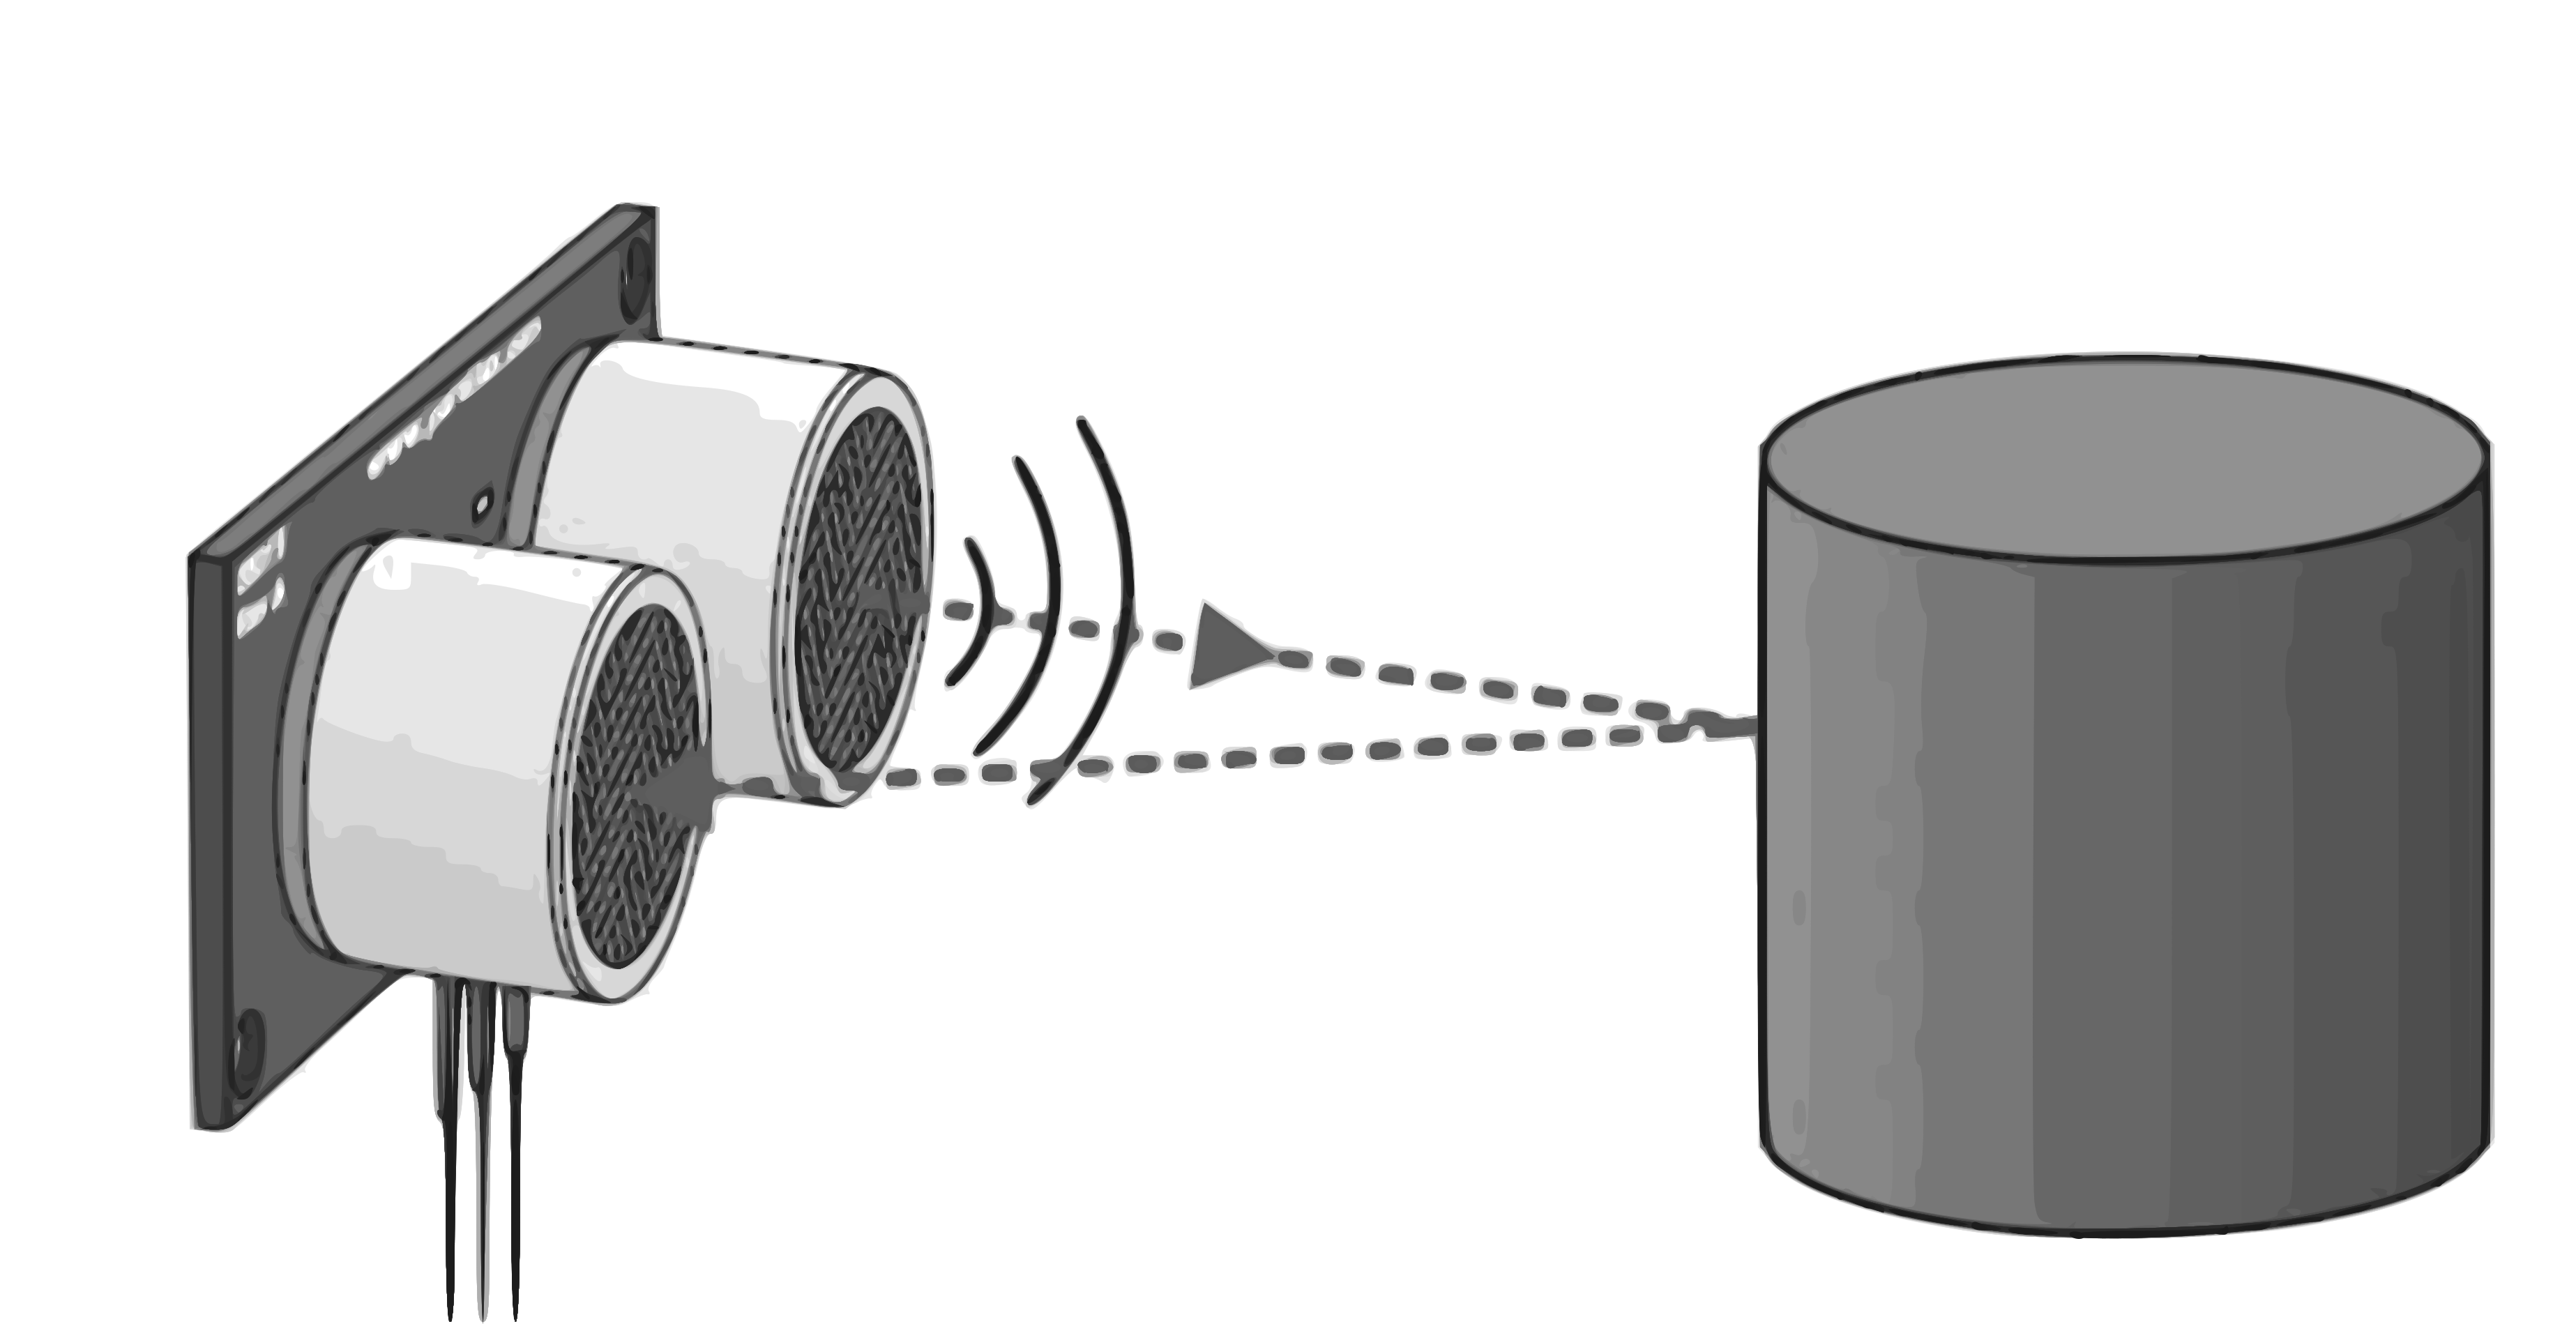
\includegraphics[width=0.7\linewidth]{secRobosMoveis/figures/ultra.png}
	\end{center}
	\caption{Funcionamento do sensor ultrassônico. Um alto-falante emite a onda sonora enquanto o outro recebe.}
	\label{fig:ultrasonico}
\end{figure}

Os métodos de estimar distâncias baseados em tempo são conhecidos por \textit{tempo de chegada} (ToA, de \textit{Time-of-Arrival}) e \textit{diferença de tempo de chagada} (TDoA, \textit{Time-Difference-of-Arrival}) \cite{savvides2001dynamic}. 
\\

Pode-se utilizar a transmissão de dois sinais simultâneos com velocidades diferentes e conhecidas para estimar distâncias. É o que se faz, por exemplo, para saber a que distância um trovão caiu. Quando um trovão aparece, dois sinais com velocidades diferentes são enviados: um sinal luminoso (que viaja a velocidade da luz) e um sinal sonoro (que viaja a velocidade do som).
Medindo a diferença entre o recebimento dos dois sinais, faz-se a estimativa da distância (veja a Figura~\ref{fig:somLuz}).

\begin{figure}[H]
	\begin{center}
		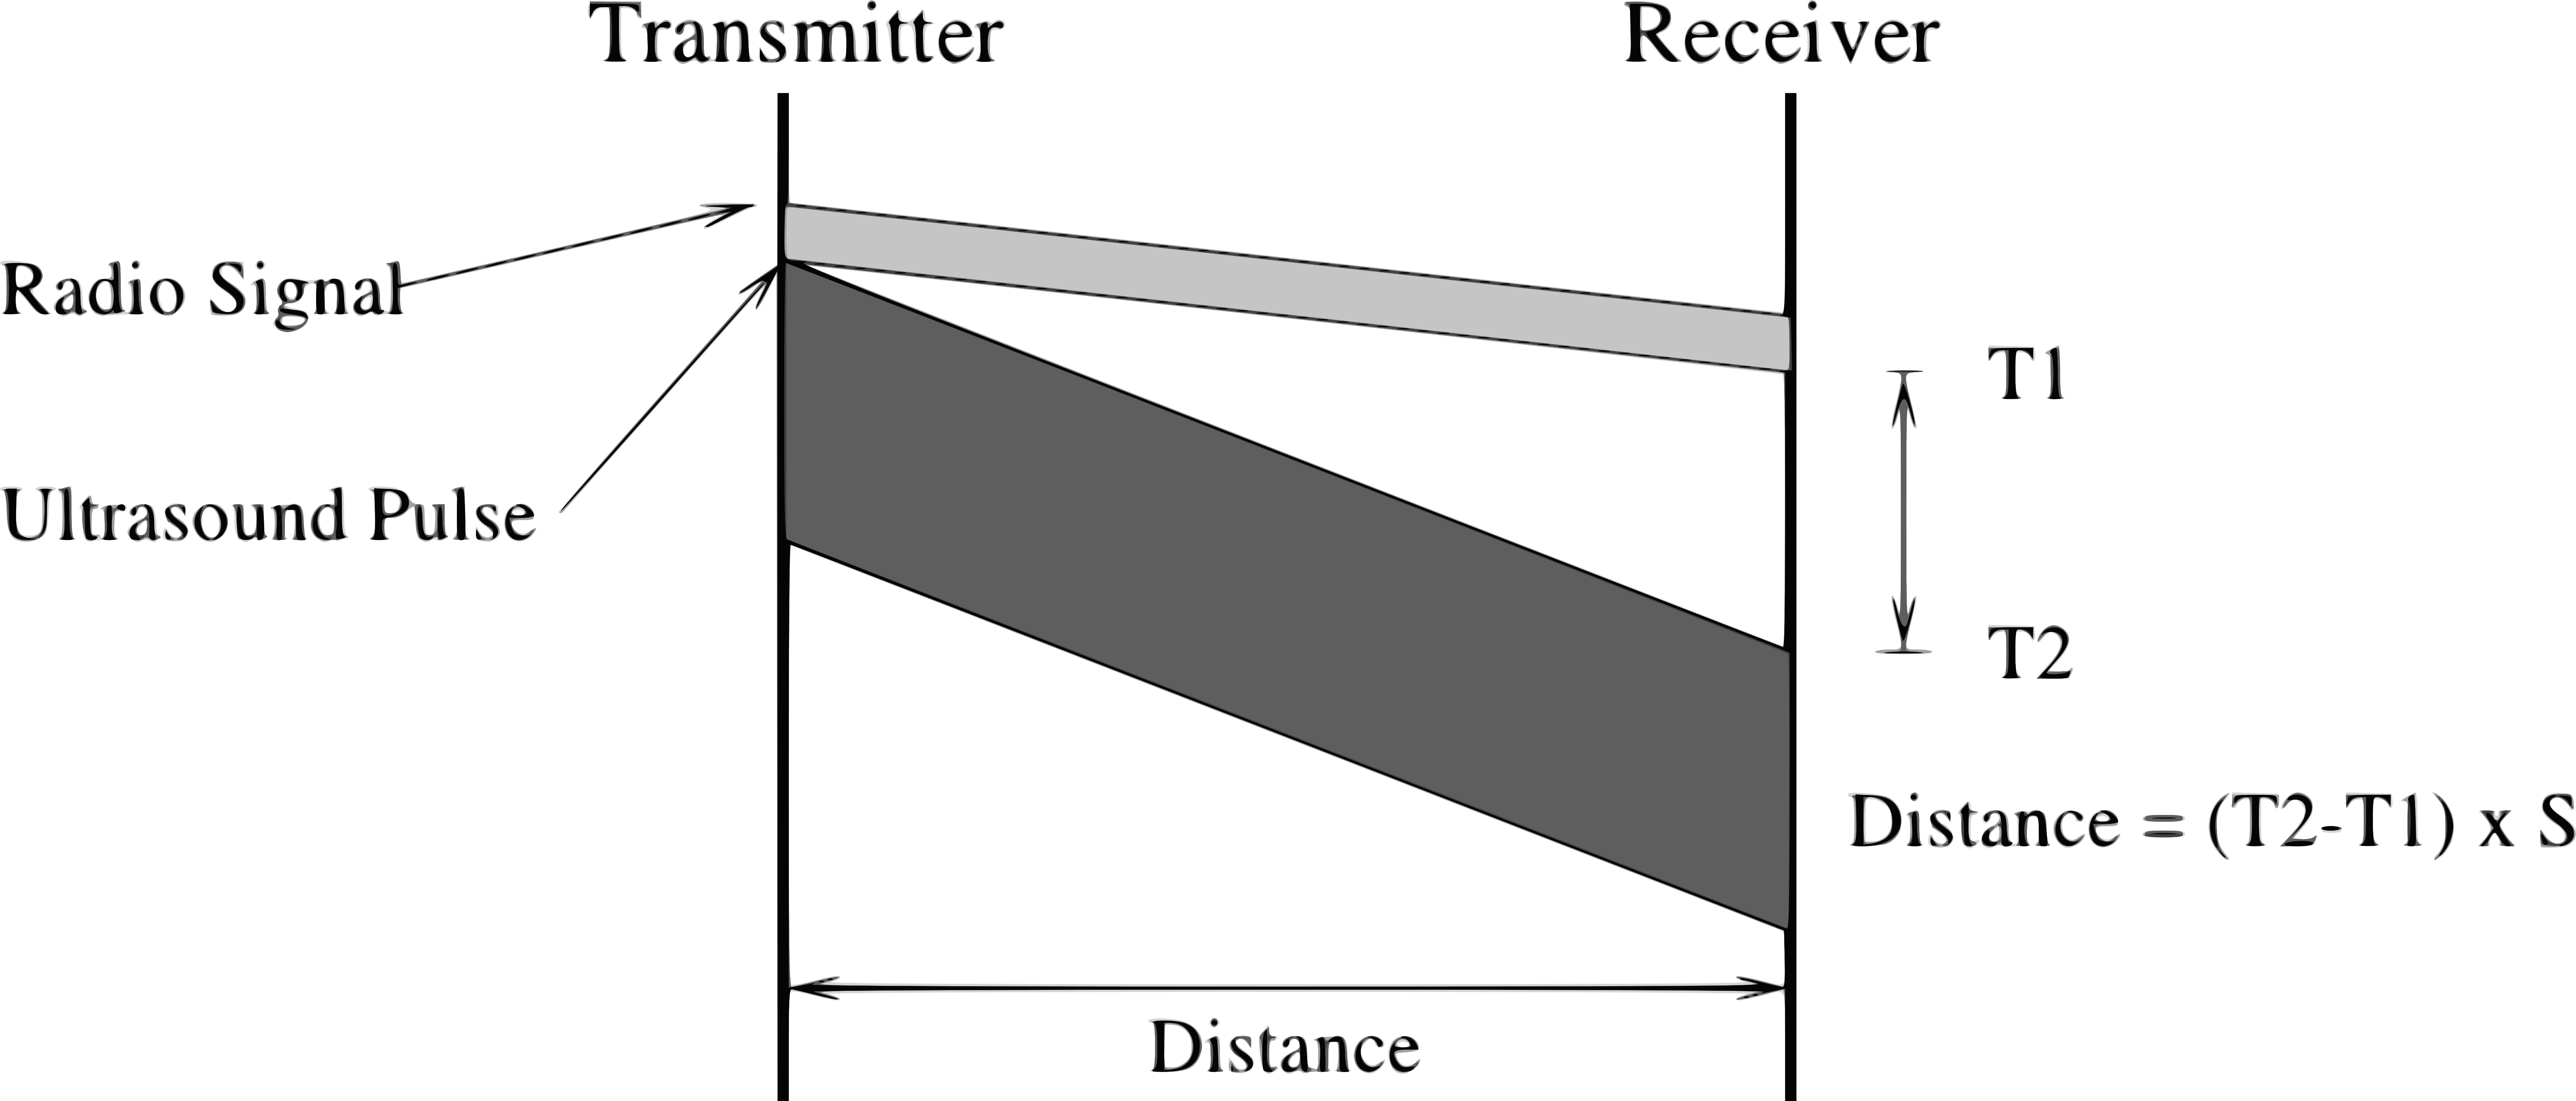
\includegraphics[width=0.7\linewidth]{secRobosMoveis/figures/somLuz.png}
	\end{center}
	\caption{Estimativa de distância usando a diferença entre um sinal ultrassônico e um de rádio \cite{savvides2001dynamic}.}
	\label{fig:somLuz}
\end{figure}

Savvides \textit{et al}. \cite{savvides2001dynamic} construíram outro protótipo, chamado Medusa, utilizando deste princípio. Para grandes distâncias, infelizmente, a utilização de sensores ultrassônicos mostrou-se ser um problema \cite{sensorsForMobileRobots}. Porém, para pequenas distâncias os resultados foram promissores, com precisões de dois centímetros para sensores separados por três metros.
\\

Em curtas distâncias, por tanto, utilizar métodos baseados em atraso do tempo de recebimento mostrou-se uma boa alternativa frente aos métodos de medição da intensidade do sinal. 

\subsection{Sobre o conjunto de sensores}

Tendo estabelecida uma forma de obter as distâncias, como discutido na seção~\ref{sec:go}, precisa-se definir um conjunto de sensores como âncoras para poder calcular a realização dos demais sensores. Afim de aplicar o Algorítimo~\ref{alg:realizacaoTrilateration}, caso o problema seja definido em $\mathbb{R}^2$ ou $\mathbb{R}^3$, precisa-se de 3 e 4 sensores como âncoras, respectivamente. Em \cite{wsnlFewAnchors}, Fekete e Jordán apresentam um estudo sobre geometrias mínimas para as âncoras que continuam garantindo a unicidade da solução.

Além disso, também deve-se garantir que estes sensores estejam próximos o suficiente para que se possa estimar distâncias (garantindo a existência de $K+1$-cliques). Por isso, deve-se pensar em um conjunto de restrições no posicionamento das âncoras e movimento dos robôs móveis de forma a garantir que sempre haverá uma ordem de $K$-lateração. Eren \textit{et al.} \cite{eren2004rigidity} apresenta um estudo sobre a realização de grafos com geometrias aleatórias. 

%Seja $d\in\mathbb{R}$ o raio máximo de obtenção de distâncias pelos sensores usados. No Algorítimo~\ref{alg:movimento}, busca-se restringir a movimentação de um robô móvel definido em um grafo $K$-laterativo, afim de perpetuar sua rigidez global.
